\documentclass[12pt, a4paper]{report}
\usepackage[T1]{fontenc}
\usepackage{times} %times new roman boring 
%\usepackage{ebgaramond-maths}
\usepackage{parskip}
\usepackage{lmodern}
\usepackage{graphicx}
\usepackage{setspace}
\usepackage{enumitem}
\setlist[enumerate]{nosep}
\usepackage{titlesec}
\usepackage{hyperref}
\setlength{\parindent} {0pt}
\renewcommand{\contentsname}{Table of Contents}
\makeatletter
\def\@makechapterhead#1{%
  %\vspace*{50pt}%
  {  \MakeUppercase{\ifnum \c@secnumdepth >\m@ne
        \fontsize{16pt}{1}\bfseries \@chapapp \space \thechapter\vspace{5pt}\\
    \fi
    \interlinepenalty\@M
     \bfseries #1}\par\nobreak
    %\vskip 0pt
  }}
\makeatother
\renewcommand{\labelenumi}{\roman{enumi}.}
\makeatletter
% Redefine the \chapter* header macro to remove vertical space
\def\@makeschapterhead#1{%
  %\vspace*{50\p@}% Remove the vertical space
  {\newpage \parindent \z@ \raggedright
    \normalfont
    \interlinepenalty\@M
    \center \fontsize{16pt}{1} \bfseries \MakeUppercase{#1}\par\nobreak
    %\vskip 18\p@ % adjust space after heading 18pt
  }}
\makeatother 
\usepackage[left = 1.5in, right = 1in, top = 1in, bottom = 1in]{geometry}
\titlespacing*{\section}{0pt}{0pt}{0pt} %left, top, bottom spacings
\titlespacing*{\subsection}{0pt}{0pt}{0pt}
\titlespacing*{\subsubsection}{0pt}{0pt}{0pt}
\titlespacing*{\paragraph}{0pt}{0pt}{0pt}
\titlespacing*{\subparagraph}{0pt}{0pt}{0pt}

%adjust fontsizes\ of sections
\titleformat*{\section}{\fontsize{14pt}{18pt}\bfseries}
\titleformat*{\subsection}{\fontsize{13pt}{18pt}\bfseries}
\titleformat*{\subsubsection}{\fontsize{12pt}{18pt}\bfseries}
\titleformat*{\paragraph}{\fontsize{12pt}{18pt}\bfseries}
\titleformat*{\subparagraph}{\fontsize{12pt}{18pt}\bfseries}

\setlength{\parskip}{18pt}
\linespread{1.5}
\newcommand{\submittedBy}
{
\makebox[8.5cm]{Bibek Chand\hfill[KAN078BEI002]}\\
\makebox[8.5cm]{Piriyanka Jha\hfill[KAN078BEI006]}\\
\makebox[8.5cm]{Sujal Shrestha\hfill[KAN078BEI009]}
}

\newcommand{\project}{Case}
\newcommand{\projectTitle}{Organization and Management of F1Soft} 
\newcommand{\doc}{Study}

\newcommand{\KECadjusttocspacings}
{
\setlength{\parskip}{0pt} % to remove paragraph spacing in TOC, LOF ...
\renewcommand{\baselinestretch}{0.1} % to adjust line spacing in toc
\newcommand*{\noaddvspace}{\renewcommand*{\addvspace}[1]{}}
\addtocontents{lof}{\protect\noaddvspace} %remove extra vertical space in LOF
\addtocontents{lot}{\protect\noaddvspace} %remove extra vertical space in LOT
}



\begin{document}
%front page



\begin{titlepage}
\begin{center}
{\Large \textbf{Kantipur Engineering College}}\\
{\large \textbf{Affiliated to Tribhuvan University}}\\
\large{\textbf{Dhapakhel, Lalitpur}}\\
\end{center}
\vfill
\begin{center}
\begin{figure}[h]
\centering

\includegraphics[width=25mm, height = 25mm]{images/logo.png}
\end{figure}
\vfill
\large{\textbf{[Subject Code: ME 708]}}\\ 
\large{\textbf{A \MakeUppercase{\project} \MakeUppercase{\doc} ON}}\\ 
\Large{\textbf{\MakeUppercase{\projectTitle}}}\\
\vfill	
\large{\textbf{Submitted by:}}\\
\large{\textbf{\submittedBy}}\\
\vfill
\large{\textbf{Submitted to:}}\\
\large{Er. Rabindra Khati}\\
\vfill
\large{\textbf{July, 2025}}
\end{center}
\end{titlepage}

\chapter*{Acknowledgment}
\addcontentsline{toc}{chapter}{Acknowledgment}%to include this chapter in TOC
We would like to express our sincere gratitude to all those who have contributed to the preparation of this case study. First and foremost, we are thankful to Kantipur Engineering College for providing us with the opportunity to submit this case study.

We are deeply grateful to Er. Rabindra Khati Sir, whose guidance and support were invaluable throughout the process. Their expertise and insightful feedback helped shape this case study into its final form.

We would also like to acknowledge the support and encouragement from the F1Soft family who provided us with their assistance and valuable suggestions.

\par
%to display members name under Acknowledgement
\begin{flushright}
\vskip 20pt
\setstretch{1.2}
\submittedBy
\end{flushright}

\chapter*{Abstract}
This case study explores the organizational structure, management practices, and operational dynamics of F1Soft International Pvt. Ltd., a leading fintech company in Nepal. Through a field visit and direct interaction with the company, the study examines how F1Soft functions using a vertical based model, where each product line such as eSewa and FonePay operates as an independent unit with its own CTO and technical team. The central Board of Directors governs overall strategic direction, while encouraging autonomy and innovation within each vertical. The company emphasizes standardization across teams, ensuring consistency despite technological diversity. A dedicated research and training unit supports employee onboarding and capacity building. This study aims to relate theoretical concepts of organization and management to real world practices, offering insights into how a modern, innovation driven company adapts management strategies to sustain growth in a competitive digital environment.

{
\KECadjusttocspacings
\makeatletter
\def\@makeschapterhead#1{%
  %\vspace*{50\p@}% Remove the vertical space above
  {\newpage\parindent\z@\raggedright
    \normalfont
    \interlinepenalty\@M
    \centering
    \fontsize{16pt}{20pt}\selectfont % ✅ MUST include \selectfont
    \bfseries\MakeUppercase{#1}\par\nobreak
    \vskip 18\p@ % space after heading
  }}
\makeatother

 
% defined in KECReportFormat.tex to adjust spacings
\tableofcontents
}
\chapter{Introduction}
\section{Background}
Understanding how organizations operate in the real world is a key aspect of the subject Organization and Management. This field of study focuses on how organizations are structured, how roles and responsibilities are distributed, how decisions are made, and how resources are managed to achieve goals efficiently. It also explores various management theories and their practical implications in today's dynamic business environment.

To connect these academic concepts with real-life practices, our group conducted a case study on F1Soft International Pvt. Ltd., a prominent fintech company in Nepal. Established with the aim of digitizing financial services, F1Soft has become a key player in the Nepali digital economy. The company is known for its widely used platforms such as eSewa and FonePay, and has expanded into more than 18 business verticals. With over 1200 employees and operations extending beyond Nepal to regions like Dubai, F1Soft provided us with a rich example of how modern organizations manage growth, innovation, and complexity.

Our visit to the company was intended to gain insights into how F1Soft is organized internally, how it functions on a daily basis, and how its management system supports its goals. During the visit, we observed the organizational environment and interacted with company representatives to learn about their structure, departmental coordination, leadership approach, and operational strategies.

This report is based on the findings of that visit. It attempts to explore and analyze the structure and management of F1Soft, relate it to theoretical concepts from our course, and reflect on how management principles are applied in practice. Through this case study, we aim to deepen our understanding of how a successful company operates in a competitive and technology-driven industry.

\section{Objectives}
\begin{enumerate}
    \item To understand the organizational structure and management practices of F1Soft international.
    \item To analyze leadership, motivation, and communication systems within the company.
    \item To relate theoretical concepts of organization and management to real world applications.
\end{enumerate}

\chapter{Company Profile}
\begin{figure}[h]
\centering
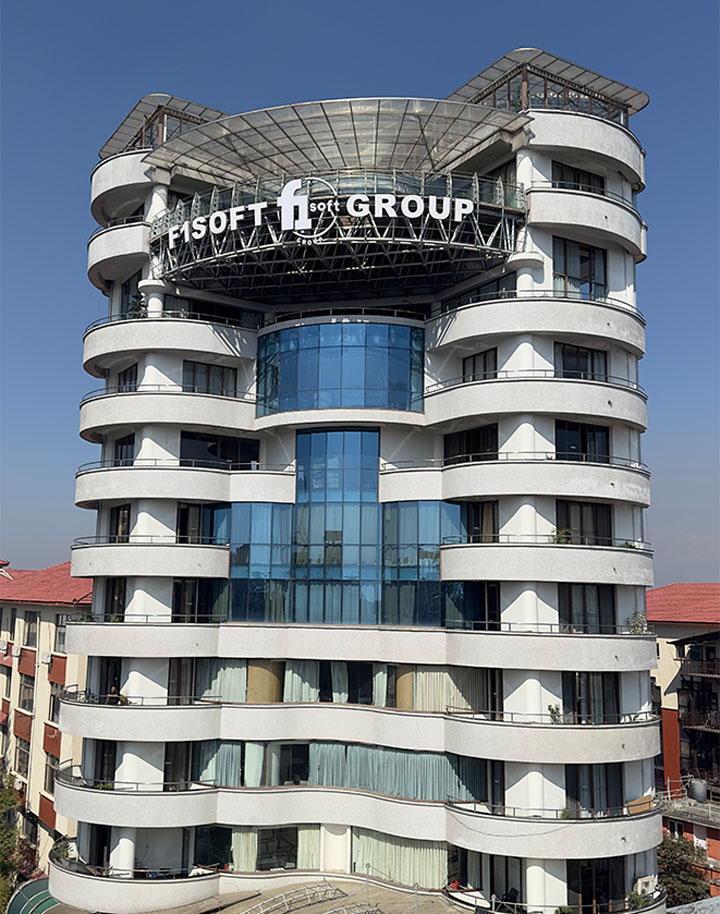
\includegraphics[scale=0.5]{images/Company-Building.jpg}
\caption{F1Soft Building}
\end{figure}
\section{Basic Information}
\begin{enumerate} 
    \item \textbf{Name}: F1Soft International Pvt. Ltd.
    \item \textbf{Headquarters}: Pulchowk, Lalitpur, Nepal
    \item \textbf{Established}: 2004
    \item \textbf{Founded by}: Bishwas Dhakal
    \item \textbf{Industry}: Financial Technology (FinTech)
    \item \textbf{Ownership}: Privately held
    \item \textbf{Employees}: 1200+
    \item \textbf{Symbol}: Tiger
    \item \textbf{Business Verticals}: 18
\end{enumerate}
\vspace{18pt}
\section{Core Products}
\begin{enumerate}
    \item eSewa
    \item FonePay
    \item FoneLoan
    \item JumJum and others.
\end{enumerate}
\vspace{18pt}
\section{Vision and Missions}
\begin{enumerate}
    \item To democratize financial services and create new possibilites for economic progress and individual prosperity.
    \item To build an inclusive digital financial ecosystem that empowers individuals and businesses through innovative technology solutions.
\end{enumerate}
\begin{figure}[h]
\centering

\includegraphics[width=25mm, height = 25mm]{images/f1softlogo.png}
\caption{F1Soft logo}
\end{figure}
\begin{figure}[h]
\centering

\includegraphics[scale=0.2]{images/tiger.jpg}
\caption{Tiger on a cliff symbol of F1Soft}
\end{figure}

F1Soft International operates as a multifaceted fintech company with a dynamic and decentralized organizational model. The company is structured around multiple business verticals, each functioning independently with its own leadership, technical team, and development strategies. Notable verticals include digital payment services like eSewa and payment switch solutions like Fonepay, among others. Each vertical is led by its own Chief Technology Officer (CTO) and adopts technologies and frameworks best suited to its domain, allowing for both agility and innovation.

Despite their operational independence, these verticals function under the strategic oversight of F1Soft’s Board of Directors, which ensures alignment with the company’s long-term vision, policies, and ethical standards. This hybrid structure of centralized governance and decentralized execution enables F1Soft to scale efficiently while encouraging innovation at the vertical level.

To maintain a consistent level of quality, security, and performance, F1Soft places strong emphasis on standardization of development processes, cybersecurity protocols, and internal operations across all its verticals. Collaboration between verticals is encouraged through regular inter-departmental coordination.

F1Soft also invests in the future of its workforce through a specialized Research and Training Unit. This unit is responsible for onboarding new employees, imparting company-standard practices, and nurturing talent through continuous professional development. It plays a critical role in maintaining the technological and cultural consistency of the organization.

Symbolized by a tiger, the company’s identity reflects strength, agility, leadership, and a bold approach to transformation. F1Soft continues to be a key player in shaping Nepal’s financial technology landscape, contributing significantly to the country’s movement toward a cashless economy.

\chapter{Organization Structure and Management}
\section{Vertical Based Organizational Structure}
A vertical-based organizational structure is a type of decentralized management model in which a company is divided into semi-autonomous units, known as verticals. Each vertical typically focuses on a specific product, service, or market segment, and functions almost like a separate business entity within the larger organization.

In such a structure, each vertical has its own leadership team, often including roles such as Chief Technology Officer (CTO), project managers, and development teams. These verticals operate independently, making decisions related to their technology stack, product development, and internal processes based on what best suits their objectives and users.

At the same time, the organization retains a central governing body—such as a Board of Directors or executive leadership—that oversees the company’s overall vision, values, and strategic alignment. This ensures that while verticals have the flexibility to innovate and respond to their specific needs, they still adhere to common standards and company-wide goals.

One of the key benefits of a vertical-based structure is agility: teams can quickly adapt to changes, innovate, and scale their products without being slowed down by bureaucracy. It also fosters specialization, as each vertical can focus deeply on its domain.

In the case of F1Soft International, this model allows various digital financial services (like eSewa and Fonepay) to operate independently while contributing collectively to the organization’s mission of leading Nepal's fintech ecosystem.
\begin{figure}
\centering
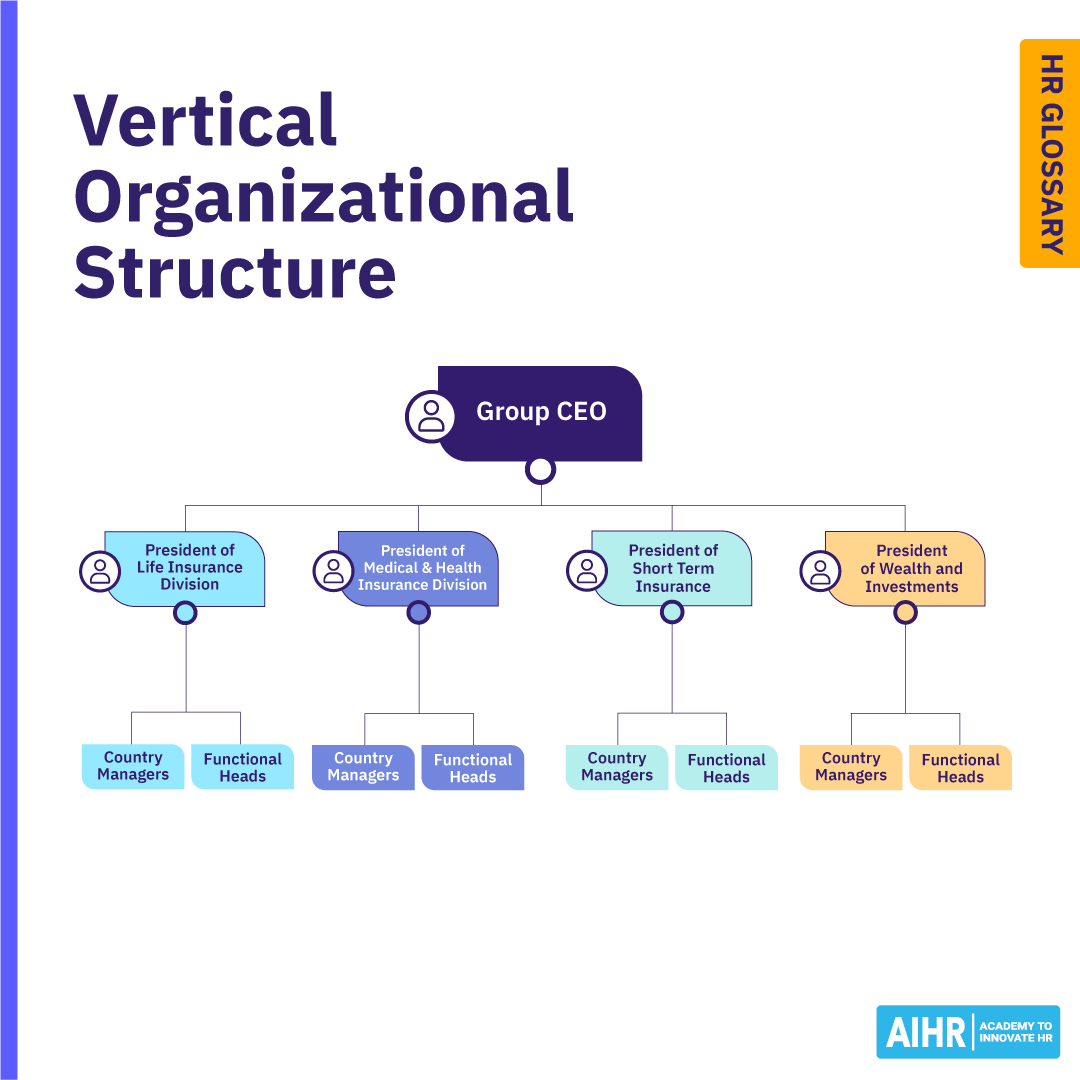
\includegraphics[scale=0.3]{images/vertical.png}
\caption{Vertical Organizational Structure}
\end{figure}
\vspace{18pt}
F1Soft International Pvt. Ltd. operates under a vertical based organizational structure, where each major product or service such as eSewa, FonePay, Foneloan, etc.functions as an independent business vertical. Each vertical is treated almost like a company within a company, with its own management, technical team, and operational strategy. This structure allows for high flexibility, specialization, and innovation within each unit.
\vspace{18pt}
\section{Vertical-Based Structure of F1Soft}
\begin{enumerate}
    \item Has its own \textbf{Chief Technology Officer (CTO)} who leads technology strategy and implementation.
    \item Operates with an \textbf{independent team} responsible for development, operations, and support.
    \item Uses \textbf{different technologies} suited to their product needs.
    \item Maintains autonomy while aligning with company-wide \textbf{standardization practices}.
\end{enumerate}
\vspace{18pt}
\section{Central Management and Governance}
\begin{enumerate}
    \item Strategic decision-making and long-term planning.
    \item Providing guidance and oversight to all business verticals.
    \item Ensuring regulatory compliance and ethical standards.
    \item Facilitating coordination and communication across the company.
\end{enumerate}
\vspace{18pt}
\section{Research and Training Division}
\begin{enumerate}
    \item Onboards new employees through structured training programs.
    \item Promotes standard practices and technological awareness.
    \item Encourages continuous learning and professional development.
\end{enumerate}
\pagebreak
\subsection{Management Philosophy}
\begin{enumerate}
    \item \textbf{Visionary} – Focused on innovation and market leadership.
    \item \textbf{Decentralized} – Empowering each vertical with decision-making authority.
    \item \textbf{Collaborative} – Promoting cooperation across teams and departments.
    \item \textbf{Standardized} – Ensuring uniformity in key processes and policies.
\end{enumerate}
This structure enables F1Soft to remain agile, innovative, and efficient, making it a leader in Nepal’s fintech industry.

\begin{figure}[h]
\centering
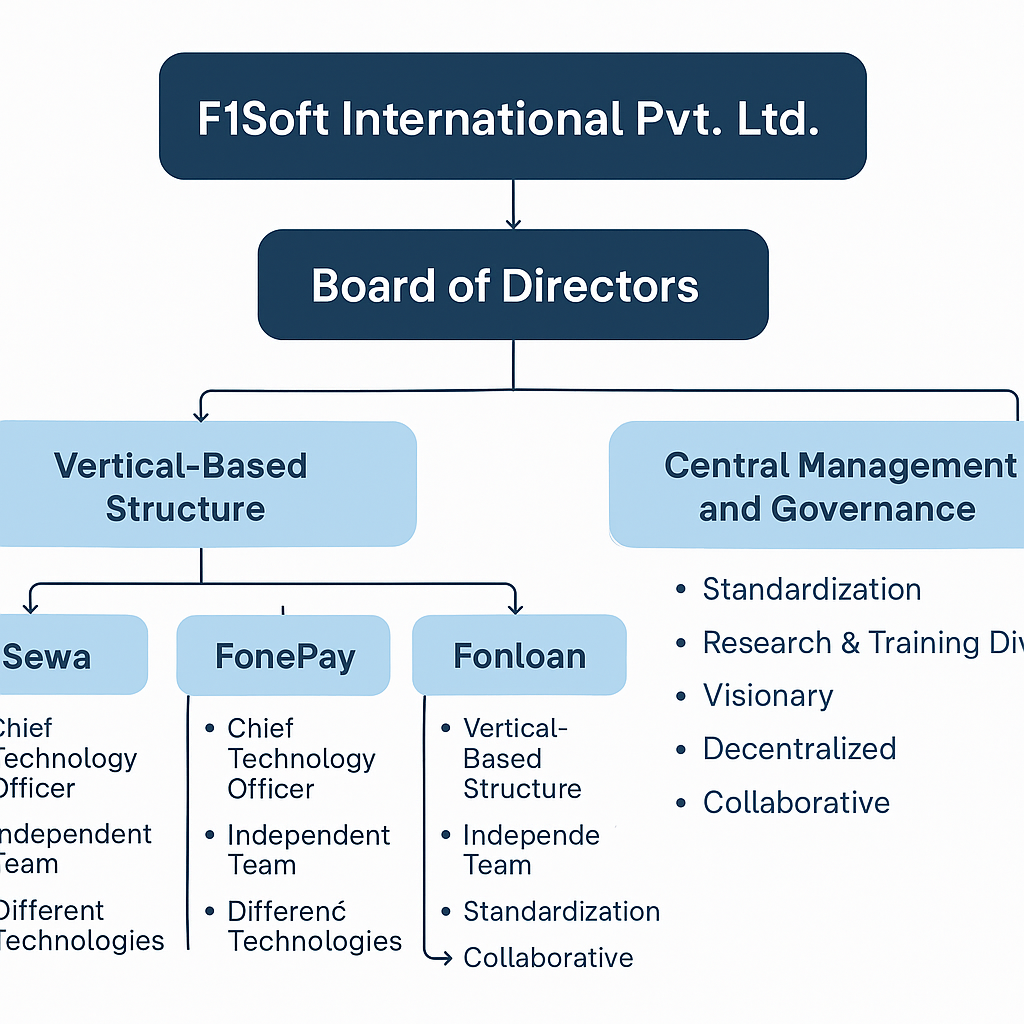
\includegraphics[scale=0.3]{images/structure.png}
\caption{Organizational Structure of F1Soft}
\end{figure}
\vspace{18pt}
\section{eSewa: A Leading Vertical of F1Soft International}
eSewa is Nepal’s first and most widely used digital wallet and payment gateway, launched under F1Soft International. Since its inception in 2009, it has transformed how individuals and businesses in Nepal conduct financial transactions. As a vertical under F1Soft, eSewa operates with a significant degree of \textbf{autonomy}, functioning like an independent company while aligning with F1Soft’s overarching strategic vision.

\begin{figure}
\centering

\includegraphics[scale=0.3]{images/esewa.png}
\caption{Esewa logo}
\end{figure}


\subsection{Organizational Structure of eSewa}
eSewa has its own leadership team, headed by a dedicated \textbf{Chief Technology Officer (CTO)} and department heads who manage product development, operations, marketing, customer service, and security. The internal hierarchy is vertical in nature, with clear lines of authority and accountability. Departments are typically divided into:

\begin{itemize}
  \item \textbf{Technology Team} – Handles app development, backend infrastructure, and platform maintenance.
  \item \textbf{Operations Team} – Manages transaction processing, vendor relationships, and partner integrations.
  \item \textbf{Business Development} – Focuses on expanding the user base and forming strategic alliances with merchants, banks, and service providers.
  \item \textbf{Customer Service} – Provides user support and handles queries through various channels.
  \item \textbf{Compliance and Risk Management} – Ensures that the platform adheres to national financial regulations and maintains cybersecurity standards.
\end{itemize}

Although these teams work independently, coordination is maintained through regular meetings and strategic reviews to ensure that efforts are aligned with F1Soft’s goals.
\vspace{18pt}
\subsection{Management Approach}
eSewa employs a flexible yet structured management style, balancing innovation with operational discipline. Agile methodologies are often used in product and software development, enabling rapid updates and new feature rollouts. Leadership emphasizes collaborative decision-making, especially in technical and product-related issues.

Team leads and department heads are given ownership of their domains, encouraging accountability and innovation. However, key policies, budgeting decisions, and long-term goals are aligned with F1Soft’s board through top-down strategic planning.

To maintain service quality and security, eSewa follows standardized practices shared across F1Soft’s verticals. These include coding guidelines, data security protocols, and user interface standards.
\vspace{18pt}
\subsection{Integration and Autonomy}
While eSewa is technically and managerially independent, it collaborates with other F1Soft verticals such as Fonepay (for interoperability) and utilizes F1Soft’s shared resources like HR and training. New employees often undergo orientation and technical workshops through F1Soft’s \textbf{Research and Training Unit}, helping to maintain cultural and technical consistency across verticals.

\bigskip

In summary, eSewa exemplifies the vertical-based model’s strength: \textit{independent operation with centralized vision}. Its success demonstrates how clear leadership, departmental autonomy, and structured coordination can lead to sustained innovation and national impact in the fintech sector.
\newpage
\section{Fonepay: Enabling Digital Payments Infrastructure}
Fonepay is another major vertical under F1Soft International, operating as Nepal’s leading interoperable payment network. It connects banks, digital wallets, and merchants across Nepal, enabling seamless QR-based payments, direct bank transfers, and real-time settlements.
\begin{figure}[h]
\centering

\includegraphics[scale=0.5]{images/fonepay.png}
\caption{Fonepay logo}
\end{figure}


\subsection{Organizational Structure of Fonepay}
Fonepay functions with autonomy similar to other verticals in F1Soft. It has its own \textbf{Chief Technology Officer (CTO)}, business leads, and operational managers. The teams are organized into the following key departments:

\begin{itemize}
  \item \textbf{Network and Integration Team} – Responsible for technical integration with banks and financial institutions.
  \item \textbf{Business Development} – Onboards new partners, merchants, and service providers.
  \item \textbf{Operations and Settlement Team} – Manages transaction flows, interbank settlements, and dispute resolution.
  \item \textbf{Compliance and Security} – Ensures adherence to regulatory frameworks and security protocols.
\end{itemize}

The teams work with a degree of specialization, maintaining Fonepay’s standards while customizing workflows for institutional partners.
\vspace{18pt}
\subsection{Management Practices}

Fonepay follows a structured, compliance-driven management style given the sensitivity and scale of financial data it handles. Decision-making is data-informed and risk-aware, involving multi-level coordination across technical, operational, and regulatory stakeholders.

The leadership encourages innovation through sandbox environments for testing new features and piloting with selected partners before full-scale implementation.
\vspace{18pt}
\subsection{Collaborative Framework}

Fonepay maintains close collaboration with the Nepal Rastra Bank and financial institutions, making its role central to the fintech ecosystem. While operating independently, it shares core technological principles and values with the broader F1Soft framework.

\bigskip

Through strong leadership and efficient operational frameworks, Fonepay has positioned itself as a national digital payment backbone, enabling safe, real-time interoperability in Nepal’s growing digital economy.
\vspace{18pt}
\section{JumJum: A Hyperlocal Delivery Platform}
\begin{figure}[h]
\centering

\includegraphics[scale=1]{images/jumjum.png}
\caption{Jum Jum logo}
\end{figure}

JumJum is a recent vertical launched by F1Soft to tap into Nepal’s growing on-demand economy. It is a hyperlocal delivery service platform that connects customers with nearby restaurants, grocery stores, and other vendors through a user-friendly mobile app.
\vspace{18pt}
\subsection{Organizational Structure of JumJum}

Though smaller than eSewa or Fonepay, JumJum operates with an agile team structure. The core departments include:

\begin{itemize}
 \item \textbf{Product and App Development} – Builds and maintains the JumJum mobile app and web portal.
  \item \textbf{Logistics and Delivery Operations} – Manages the network of delivery personnel and service efficiency.
  \item \textbf{Vendor Relations} – Onboards and supports restaurants, shops, and service partners.
  \item \textbf{Customer Support} – Handles user queries, refunds, and service feedback.
\end{itemize}

Each unit is guided by its own team lead, with support from the overarching F1Soft infrastructure for HR, compliance, and technical standards.

\vspace{18pt}
\subsection{Management and Strategy}

JumJum adopts a startup-like management culture focused on speed, adaptability, and customer-centricity. Lean methodology and rapid iteration are key features of its operational approach. 

Management promotes experimentation, A/B testing of features, and regular user feedback collection to evolve the platform. Despite its fast pace, the platform remains tethered to F1Soft’s principles on data security, reliability, and ethical business practices.

\vspace{18pt}
\subsection{Synergy within F1Soft}

JumJum benefits from integration with F1Soft’s payment and logistics technologies. It leverages eSewa for digital payments and collaborates with Fonepay for future interoperability goals. Additionally, the training and research support from F1Soft helps scale operational capacity as JumJum grows.

\bigskip
JumJum represents F1Soft’s expansion into consumer services beyond finance. With a vertical-based agile team and strong integration with the parent ecosystem, it is strategically positioned to grow in Nepal’s evolving e-commerce landscape.

\chapter{Conclusion}
The case study on F1Soft International has provided valuable insights into how a leading fintech company in Nepal operates using a vertical-based organizational structure. Through our visit and analysis, we observed that F1Soft functions as a parent organization with multiple autonomous verticals such as eSewa, Fonepay, and JumJum, each operating under its own management while aligning with the core values and strategic vision of the company.

F1Soft emphasizes decentralization for agility and innovation, while maintaining oversight through a central board of directors. Each vertical, with its own CTO and dedicated teams, follows distinct technological and managerial practices suited to its domain, whether it be digital payments, interoperable banking, or last-mile delivery services. Despite their autonomy, these verticals maintain coherence through shared standards, unified branding, and cross-functional collaboration.

The company’s investment in employee training, research, and continuous improvement reflects a forward-thinking approach to organizational development. Its focus on standardization alongside innovation makes F1Soft a benchmark for managing diverse technology-driven business units in a fast-changing industry.

In conclusion, the visit to F1Soft has enabled us to connect theoretical frameworks of organization and management with real-world applications, providing a practical perspective on how modern Nepali enterprises are structured and governed for sustained growth.
\end{document}
